%----------------------------
\chapter{System Architecture}
%----------------------------
\label{cha:architecture}
This chapter describes the architecture of our system. The system is build as
a decision support system for practitioners at a hospital. To prevent any
confusion, two roles are introduced.
\begin{description}
	\item[User] Practitioner that uses the system to search for relevant
				therapy chapters for a given patient case.
	\item[System administrator] Computer savvy personnel, in this case us, that
				manages the system. Doing the parsing of input files and
				building indices.
\end{description}

Our system consist of three logical parts: Python modules, input files, and
output files. There is also the external Python library Whoosh, used for
indexing and searching. In the following sections, each part will be explained
in detail. For an outline of the system, see \autoref{fig:systemarch}.

\begin{figure}[tbp]
	\noindent\makebox[\textwidth]{%
	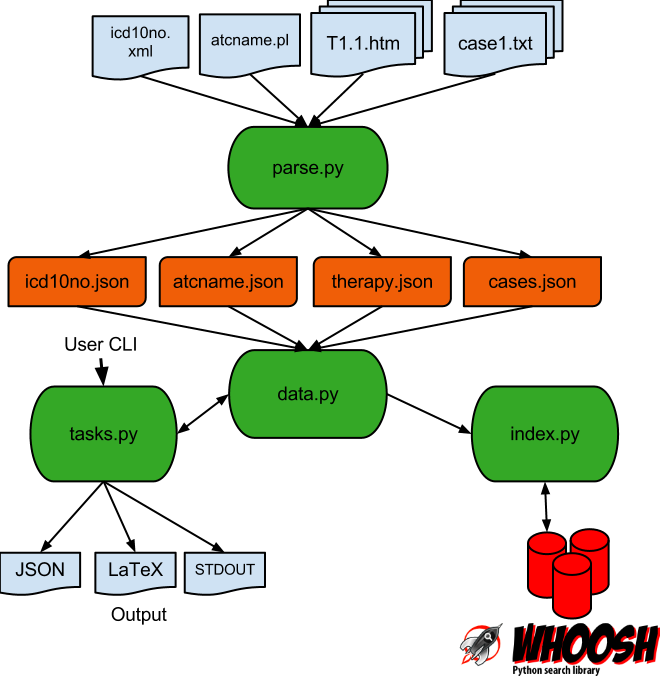
\includegraphics[width=1.1\textwidth]{./img/system_architecture2}}
	\caption{System overview\label{fig:systemarch}}
\end{figure}


\section{Whoosh}
%---------------
Whoosh\footnote{Whoosh: \url{http://pypi.python.org/pypi/Whoosh}} is a
search-engine library written in Python to support fast indexing and searching
of text collections. The library provides high performance, multifunctional
queries and support for scoring algorithms.

We use it to store, index and search on the four types of input data we must
handle: ICD-10 codes, ATC codes, therapy chapters, and patient cases. We only
use Whoosh search functionality for the first two tasks.


\section{Python modules}
%-----------------------
The system consists of four Python modules: parse.py, data.py, index.py, and tasks.py. Each module has its own features and tasks, and together they form the functional core of the system. An additional Python library, Whoosh, provides the core index and search functionality. In the following paragraphs each module is described in greater detail. For a full overview of the modules with their associated classes, attributes and methods, see the system's class diagram in \autoref{fig:classdiag}.

\begin{figure}[tbp]
	\noindent\makebox[\textwidth]{%
	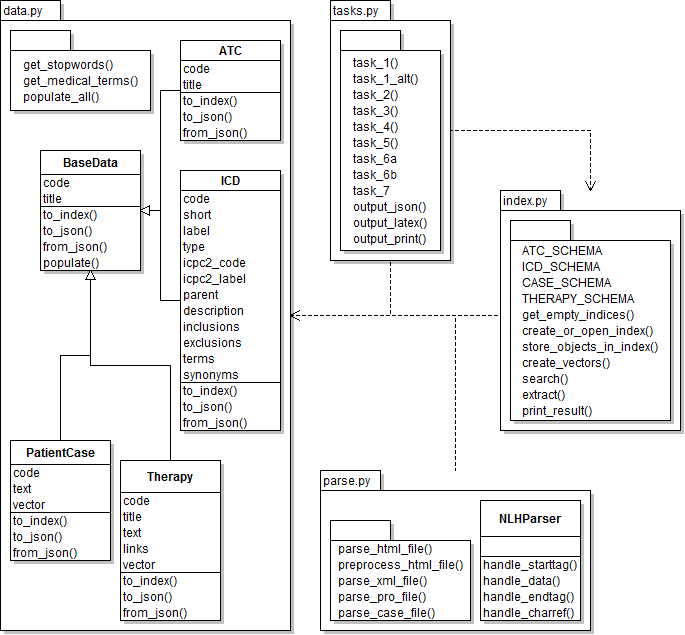
\includegraphics[width=1.1\textwidth]{./img/class_diagram}}
	\caption{Class diagram of the Python modules\label{fig:classdiag}}
\end{figure}

\paragraph{parse.py}
This module preprocess and converts input files to the more preferred JSON format, which gives better readability and reduces complexity for the following modules, which now only have to support one type of file. The module supports multiple file formats as input, for further information see the input files section \ref{inputfiles}. The module is especially important for stripping out all the HTML tags from the therapy chapters. 

\paragraph{data.py}
The JSON files created by the parse module, are used as input to the data module. The data module holds representation of all the data the system needs. As a basis for holding the data we have the BaseData class, which is inherited by more specific classes for the different representations. As the system loads a JSON file, it determines which representation that should be used, ICD, ATC, PatientCase or Therapy. 

\paragraph{index.py}
Main module for building and managing the indices. After the data module has created the representation and holds the data, the index module can build indexes of it. This gives the system the ability to store text and to search for terms.

\paragraph{tasks.py}
This module contains the Command Line Interface (CLI), which makes the user able to interact with the system. The module contains methods to perform and solve the different tasks of the assignment, specified by the user. Output is generated by this module, either as STDOUT print or as a JSON- or LaTeX-file. Sample output can be seen in the appendices. 


\section{Input files}
%--------------------
\label{inputfiles}
The system needs to support multiple file formats to be able to preprocess and parse the files given in the assignment. The ICD-10 file is a .xml file, the ATC file is a .pro file, the Norsk Legemiddel Håndbok is HTML and the cases are .txt files. So the parse module has support for: xml, pro, htm and txt. 


\section{Output files}
%---------------------
The result of the system is always presented in the command line. To be able to store the results and present them in this report, it was necessary and beneficial for us to make an output feature. The system is able to print the results to a JSON- or LaTeX-file. 


